%!TEX TS-program = xelatex
\documentclass{beamer}

\usepackage{HSE-theme/beamerthemeHSE} % Подгружаем тему

%%% Работа с русским языком и шрифтами
\usepackage[english,russian]{babel}   % загружает пакет многоязыковой вёрстки
\usepackage{fontspec}      % подготавливает загрузку шрифтов Open Type, True Type и др.

%% % \defaultfontfeatures{Ligatures={TeX},Renderer=Basic}  % свойства шрифтов по умолчанию
%% % \setmainfont[Ligatures={TeX,Historic}]{KanjiStrokeOrders.ttf} %  установите шрифты Myriad Pro или (при невозможности) замените здесь на другой шрифт, который есть в системе — например, Arial
%% \setmainfont[ExternalLocation={./}]{MyriadPro-Regular.otf} %  установите шрифты Myriad Pro или (при невозможности) замените здесь на другой шрифт, который есть в системе — например, Arial
%% \setsansfont[ExternalLocation={./}]{MyriadPro-Regular.otf}% {CourierNew}  %  установите шрифты Myriad Pro или (при невозможности) замените здесь на другой шрифт, который есть в системе — например, Arial
%% \setmonofont[ExternalLocation={./}]{MyriadPro-Regular.otf} {Courier New}

\defaultfontfeatures{Ligatures={TeX},Renderer=Basic}  % свойства шрифтов по умолчанию
% \setmainfont[Ligatures={TeX,Historic}]{KanjiStrokeOrders.ttf} %  установите шрифты Myriad Pro или (при невозможности) замените здесь на другой шрифт, который есть в системе — например, Arial
\setmainfont[ExternalLocation={./},Ligatures={TeX,Historic}]{MyriadPro-Regular.otf} %  установите шрифты Myriad Pro или (при невозможности) замените здесь на другой шрифт, который есть в системе — например, Arial
\setsansfont[ExternalLocation={./}]{MyriadPro-Regular.otf} %  установите шрифты Myriad Pro или (при невозможности) замените здесь на другой шрифт, который есть в системе — например, Arial
\setmonofont{Courier New}

\uselanguage{russian}
\languagepath{russian}
\deftranslation[to=russian]{Theorem}{Теорема}
\deftranslation[to=russian]{Definition}{Определение}
\deftranslation[to=russian]{Definitions}{Определения}
\deftranslation[to=russian]{Corollary}{Следствие}
\deftranslation[to=russian]{Fact}{Факт}
\deftranslation[to=russian]{Example}{Пример}
\deftranslation[to=russian]{Examples}{Примеры}

\usepackage{multicol} 		% Несколько колонок
\graphicspath{{images/}}  	% Папка с картинками

%%% Информация об авторе и выступлении
\title[Заголовок]{Заголовок презентации} 
\subtitle{Подзаголовок презентации / Название конференции}
\author[Имя автораwwwwwwww]{Абрамов Артем \\ \smallskip \scriptsize \url{author@hse.ru}\\\url{http://hse.ru/staff/author/}}
\institute[Высшая школа экономики]{Национальный исследовательский университет \\ «Высшая школа экономики» (Москва)}
\date{\today}

\begin{document}	% Начало презентации

\frame[plain]{\titlepage}	% Титульный слайд

\section{Просто слайд с текстом}
\subsection{Просто слайд с текстом}

\begin{frame}
\frametitle{Просто слайд с текстом}
	\emph{Высшая школа экономики} "--- исследовательский университет, осуществляющий свою миссию через научно-образовательную, проектную, экспертно-аналитическую и социокультурную деятельности на основе международных научных и организационных стандартов. Мы осознаем себя частью мирового академического сообщества, считаем международное партнерство, вовлеченность в глобальное университетское взаимодействие ключевыми элементами нашего движения вперед. Будучи российским университетом, мы работаем на благо России и ее граждан.
\end{frame}

\begin{frame}
\frametitle{Список}
\framesubtitle{Нумерованный список}
	\begin{enumerate} 
		\item Первый пункт:
		\begin{itemize}
			\item подпункт 1;
			\item подпункт 2.
		\end{itemize}
		\item Второй пункт
		\begin{enumerate}
			\item нумерованный подпункт.
		\end{enumerate} 
		\item Третий пункт
	\end{enumerate} 
\end{frame}

\begin{frame}
\frametitle{Список}
\framesubtitle{Маркированный список}
	\begin{itemize}
		\item Первый пункт:
		\begin{itemize}
			\item подпункт 1;
			\item подпункт 2.
		\end{itemize}
		\item Второй пункт
		\begin{enumerate}
			\item нумерованный подпункт.
		\end{enumerate}
		\item Третий пункт
	\end{itemize}
\end{frame}

\begin{frame}
\frametitle{Слайд с двумя колонками текста}
	\begin{multicols}{2}
			\begin{enumerate} 
		\item Первый пункт:
		\begin{itemize}
			\item подпункт 1;
			\item подпункт 2.
		\end{itemize}
		\item Второй пункт
		\begin{enumerate}
			\item нумерованный подпункт.
		\end{enumerate} 
		\item Третий пункт
	\end{enumerate} 
	\columnbreak
	\begin{itemize}
		\item Первый пункт:
		\begin{itemize}
			\item подпункт 1;
			\item подпункт 2.
		\end{itemize}
		\item Второй пункт
		\begin{enumerate}
			\item нумерованный подпункт.
		\end{enumerate}
		\item Третий пункт
	\end{itemize}
	\end{multicols}
\end{frame}

\begin{frame}
\frametitle{Слайд с картинкой}
	\begin{multicols}{2}
		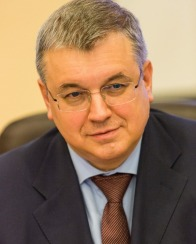
\includegraphics[width=\columnwidth]{kouzminov.png}
		\columnbreak
		До 2014 года в ВШЭ было порядка 40 факультетов и отделений. Весной 2014 года начаты структурные реформы: в университете создаются «большие» факультеты («мегафакультеты»).
		\medskip 

		\textbf{\textit{Ректор}} \\ Высшей школы экономики "--- \alert{Ярослав Иванович Кузьминов}
	\end{multicols}
\end{frame}

\begin{frame}
\frametitle{Блоки}
	\begin{theorem}[Пифагора]
		Если $a$ и $b$ "--- длины катетов прямоугольного треугольника, а~$c$ "--- длина гипотенузы, то $a^2+b^2=c^2$.
	\end{theorem}

	\begin{alertblock}{Блок с красным заголовком}
		Содержимое.
	\end{alertblock}

	\begin{exampleblock}{Блок с зеленым заголовком}
		Содержимое.
	\end{exampleblock}
\end{frame}

\begin{frame}[c]
\begin{center}
\frametitle{\LARGE Спасибо за внимание!}

{\LARGE \inserttitle}

\bigskip

{\insertauthor} 

\bigskip\bigskip

{\insertinstitute}

\bigskip\bigskip

{\large \insertdate}
\end{center}
\end{frame}

\end{document}
